\documentclass[11pt]{article}

% MOTOR paper, first draft (#98). Same class, packages, margins and bibliography style as SCORE's paper
% (paper/arxiv/main.tex). Build: tectonic -X compile main.tex (paper/CLAUDE.md).
% Rules carried over from paper/CLAUDE.md: every number is read from a source named in a comment beside it;
% wherever final content will go, a gap box of the final size stands in its place; numbers still moving are
% marked [interim].
\usepackage{iftex}
\ifPDFTeX
  \usepackage[T1]{fontenc}
  \usepackage[utf8]{inputenc}
  \usepackage{lmodern}
  \usepackage{textcomp}
\else
  \usepackage{fontspec}
\fi
\usepackage{amsmath,amssymb}
\usepackage{longtable,booktabs,array,calc}
\usepackage{graphicx}
\usepackage{xcolor}
\usepackage[numbers,sort&compress]{natbib}
\usepackage{microtype}
\usepackage{placeins}
\usepackage{caption}
\captionsetup{font=small,skip=4pt}
\usepackage[margin=2.5cm]{geometry}
\usepackage[colorlinks=true,linkcolor=blue,citecolor=blue,urlcolor=blue]{hyperref}
\setlength{\emergencystretch}{3em}
\makeatletter\def\fps@figure{tp}\def\fps@table{tp}\makeatother
\renewcommand{\topfraction}{0.9}\renewcommand{\textfraction}{0.1}\renewcommand{\floatpagefraction}{0.8}
\setlength{\textfloatsep}{10pt plus 2pt minus 2pt}

% A gap: a box of the final figure's or table's size, saying what goes there and what it waits on.
\newcommand{\gapbox}[3]{%
  \noindent\fbox{\parbox[c][#2][c]{\dimexpr#1-2\fboxsep-2\fboxrule\relax}{\centering\small\setlength{\parskip}{3pt}%
  \textbf{Gap:} #3}}}
% A number that will still change.
\newcommand{\interim}{\textsuperscript{\textcolor{red}{[interim]}}}
\newcommand{\dg}{\ensuremath{^\circ}}

\title{MOTOR: Musculoskeletal Optimisation Through Open Robotics Simulation}
\author{J.P. Kardolus, Babon Innovations B.V., Utrecht, The Netherlands}
\date{Working draft, 7 November 2026}

\begin{document}
\maketitle

\begin{abstract}
\noindent MOTOR is an open chain from one ordinary video to the ground reaction force under each foot, the joint
moments and the force in each of 416 muscles, on one GPU. A monocular estimator gives a parametric body per frame; a
full-body musculoskeletal model is fitted to it and stood on the floor the camera sees; a residual reduction makes the
movement agree with the ground; and a two-stage static optimisation gives the ground reaction force, then the muscle
activations. Every stage runs on Newton and MuJoCo Warp, deterministically. It takes a median 66\,s per trial on one
card, where OpenCap's recorded solves take 44 to 70\,min on the CPU. On OpenCap's LabValidation cohort (715 of 720
single-camera inputs) the matched joint angle error is 5.16\dg{} (centred 3.06\dg). On the five subjects never used
to choose a setting, the vertical force per foot follows the plates with a median correlation of 0.78 and 0.79, and
the vertical ground reaction force error fell from 54 to 16\% body weight (11.6\% on the 45\dg{} camera; OpenCap's
two cameras: 11.4\%). Joint moments (2.4\% weight times height, OpenCap 1.2) and the pelvis residual are not yet at
the lab's level. MOTOR is open source under the MIT licence.
\end{abstract}
% Every number: paper/evidence/sim-body/labval-final-2026-11-07.txt; OpenCap's solves (squats1 2635 s, walking1
% 4196 s): #98 comment "Timing comparison".

\section{Introduction}

Joint angles from video are now close to laboratory accuracy with one or two smartphones
\cite{uhlrich2023opencap,gilon2026monocular,peiffer2025pbl,kardolus2026direct}. The force under each foot and in each
muscle still comes from a slow CPU pipeline in OpenSim \cite{delp2007opensim,rajagopal2016fullbody,dembia2020moco};
OpenCap brought it to smartphone video, at tens of minutes of solving per trial \cite{uhlrich2023opencap}.

Much of what MOTOR does was shown first by others. Cotton fitted biomechanical models to video as differentiable
models in MuJoCo on the GPU \cite{cotton2024differentiable}; the Portable Biomechanics Laboratory fits one body scale
jointly across all of a person's trials from a handheld phone \cite{peiffer2025pbl}; KinTwin recovers torques, muscle
activations and ground reaction forces from markerless capture \cite{cotton2025kintwin}; and Cotton et al.\ fit a
person's constants over frames sampled from all their recordings \cite{cotton2026b3d}, an idea MOTOR's fit uses.
MyoSuite \cite{caggiano2022myosuite} provides the muscle model, LocoMuJoCo \cite{alhafez2023locomujoco} and MuJoCo
\cite{todorov2012mujoco} the simulation lineage; MuscleMimic \cite{li2026musclemimic} and MS-Emulator
\cite{wei2026mshuman} run bodies of 400 to 700 muscles on MuJoCo Warp, and static optimisation on MuJoCo models has
run on the CPU \cite{chauhan2026fatigue,verma2025emg2tendon}.

MOTOR's own part is narrow, and its case is speed and depth: the whole chain from video to muscle forces (fit,
footing, residual reduction, ground reaction force per foot, two-stage static optimisation) on MyoFullBody's 416
muscles, every stage on one GPU in about a minute per trial, bit-for-bit repeatable, and validated on a public cohort
on forces, moments and muscles as well as angles. To our knowledge it is the
first open chain from video to muscle forces on Newton \cite{newton} and MuJoCo Warp \cite{mujocowarp}. It is the
sim body of SCORE, an open environment synthesis framework, run here on real video.
% Novelty search and allowed claim: #98 comment "Newton novelty" (2026-11-06).

\begin{figure}[t]
\centering
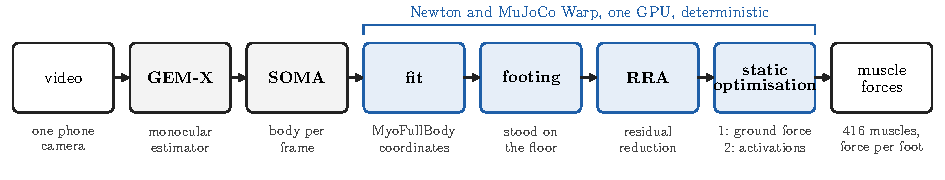
\includegraphics[width=\linewidth]{figures/pipeline.pdf}
\caption{MOTOR's chain from one video to muscle forces. The stages in blue run every frame at once on one GPU.}
\label{fig:pipeline}
\end{figure}

\section{Method}

\paragraph{From video to a body.} GEM-X \cite{gemx,li2025genmo} turns the video into a SOMA body
\cite{saito2026soma} per frame at 30\,Hz, keeping its identity, root translation and global segment rotations. SOMA
is the truth: its shape and pose are never changed. GEM-X is given the camera's field of view that MoGe-2
\cite{wang2025moge2} estimates from the same video, and its own contact post-process holds the static feet. Its world
has no floor, so the floor is seen instead: fitted to MoGe-2's floor points beside the person, the clip is turned onto
it in one rigid turn and lowered until its feet's lowest point meets it.
% tools/labval/_soma.py and tools/labval/CLAUDE.md (worktree labval-adapter, commit d6ac3b5d); field of view and seen
% floor: tools/labval/CLAUDE.md ("The floor is seen, not assumed"), commits 58c54d6f and 292d6f88 (#98).

\paragraph{Fit.} The body is MyoFullBody \cite{caggiano2022myosuite} (arm and hand from MoBL-ARMS
\cite{holzbaur2005upper,saul2015benchmarking}): 416 muscles, 86 bones and 131 joints, 95 of them free. Its bone groups
are sized to the person's SOMA body and its masses spread by SOMA's segment volumes over the subject's measured mass.
One solver fits the person's constants once, on frames sampled across the recordings \cite{cotton2026b3d}, then every
frame's joint angles against each SOMA segment's rotation, 84 anatomical landmarks on the SOMA skin and SOMA's joints,
with the model's joint couplings held exactly and a cost that keeps the bones inside the skin. On the card it
equals the CPU reference (mink \cite{mink}) within 0.01\dg{} and 0.01\,mm.
% Counts: paper/evidence/sim-body/model-2026-11-06.txt. Landmarks: score/stages/sim_body/inside/landmarks/CLAUDE.md.
% Constants: score/stages/sim_body/inside/fit/__init__.py. Card equals mink: commit 9dfd12b1.

\paragraph{Footing and ground.} The standing feet are stood on the floor by moving the whole body up or down, never by
changing the pose, and GEM-X's vertical drift between flights is taken off the root alone. The ground is what the camera sees: the floor, a sit-to-stand's 40\,cm chair
\cite{uhlrich2023opencap} and a drop jump's box, each a drawn surface. It pushes only on points of the person's SOMA
skin, carried by the bones, that touch it; a foot GEM-X sees standing is pushed from its sole up to 5\,cm. That
height, the 5\,mm contact gap and the force share between feet are the only settings chosen on LabValidation: on
subjects 2 to 5 against their plates, never against angles.
% score/stages/sim_body/CLAUDE.md (contact on SOMA's skin, Skin.credited up to 5 cm); tools/labval/CLAUDE.md (seen
% stance, drift, chair and box); commits a40b66d6, 3504c3ed, 9c6c5fb9, 53b5fc9f; tuning arms A to E on subjects 2-5:
% paper/evidence/sim-body/labval-final-2026-11-07.txt ("tuning").

\paragraph{Forces.} Per frame, inverse dynamics gives the generalised forces the movement needs. A residual reduction in the manner of OpenSim's RRA first adjusts the pelvis,
trunk and masses within a per-frame cap so that the ground explains the movement. The forces are then split in the two
stages of OpenSim's static optimisation \cite{delp2007opensim}: the ground reaction force from the pelvis' six balance
equations alone, then the muscle activations with that force fixed. A knee's small free turn is carried by its
ligaments, so it no longer splits the vasti. Solved together the problem was ill-posed (a
$10^{-6}$ nudge moved an activation by up to 1.0; in two stages, by at most $5\times10^{-3}$). What
force remains at the pelvis is recorded as the residual, judged against 2\% of body weight and 1\% of weight times
centre-of-mass height \cite{hicks2015model}, and never applied.
% score/stages/sim_body/CLAUDE.md (two stages, RRA, residual limits); commit f8e0d3f7 (nudge 1.0 to 5e-3);
% ligaments: commit 7fdd234b.

\paragraph{One GPU, repeatable.} Every stage runs every frame at once on the card with MuJoCo Warp inside Newton,
in Warp's \cite{warp} deterministic mode: two runs agree bit for bit, which answers, for this chain, the CPU against
GPU drift reported on MyoSuite bodies \cite{mujocowarp1835}.
% Bit for bit: commit e0c46164 and paper/evidence/sim-body/speed-2026-11-06.txt (same.py lines).

\begin{figure}[t]
\centering
\begin{minipage}[c]{0.3\linewidth}\centering
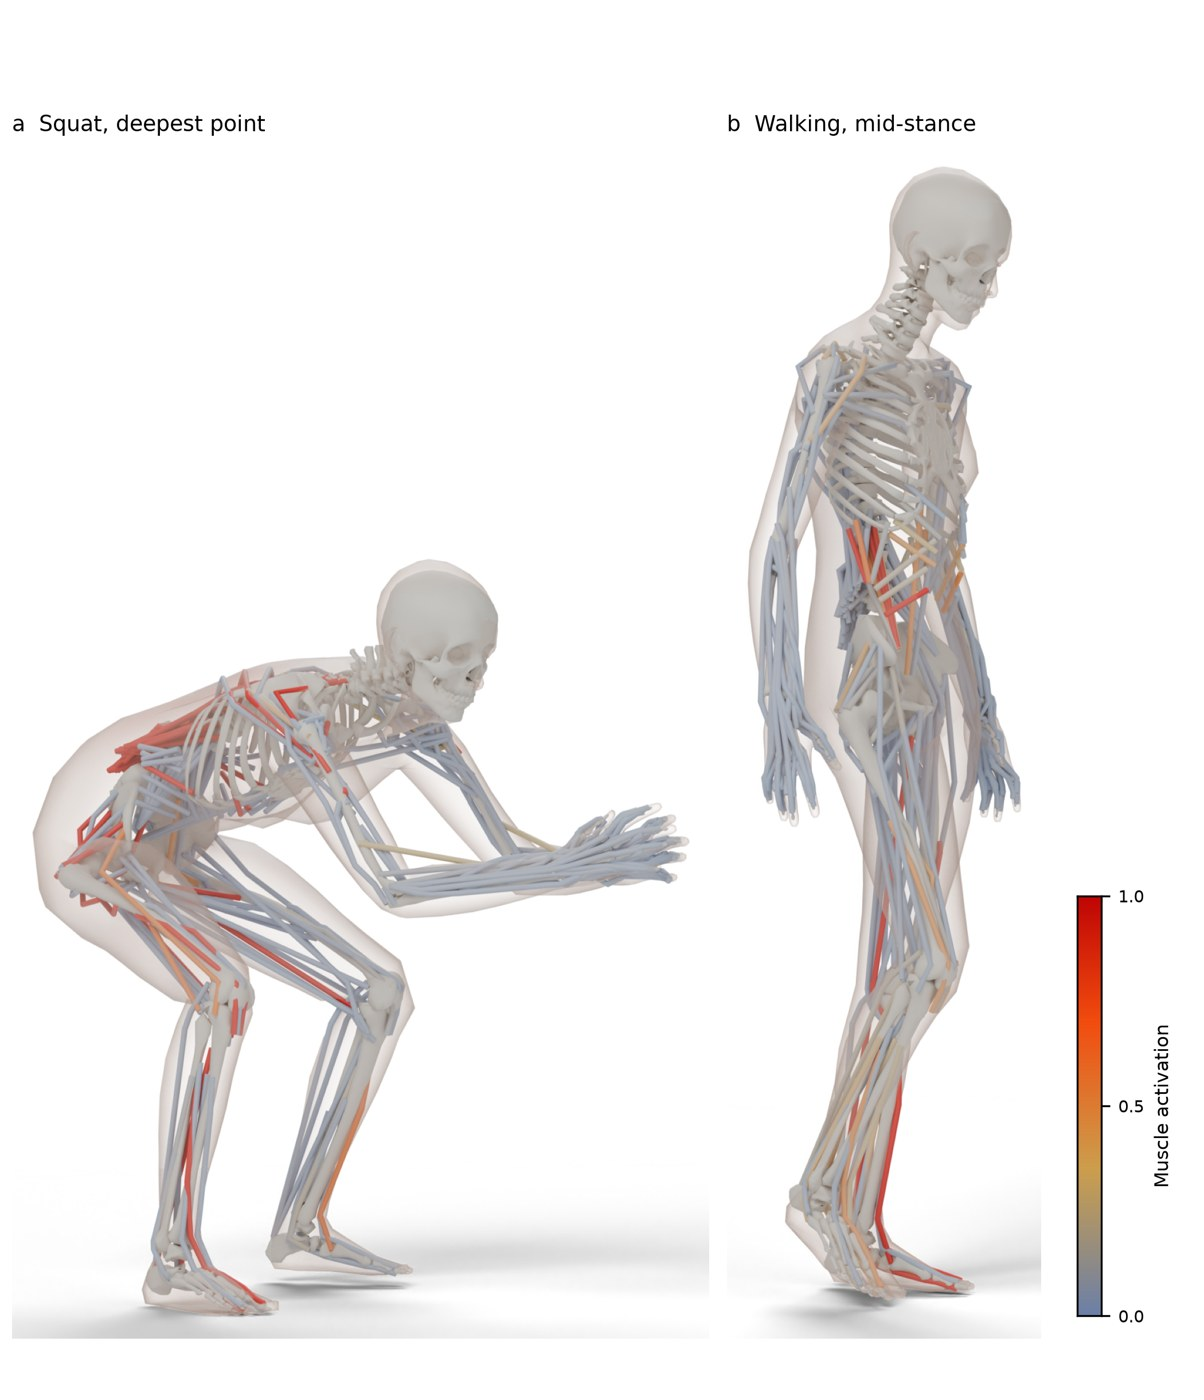
\includegraphics[width=\linewidth]{figures/simbody-in-skin.jpg}
\end{minipage}\hfill
\begin{minipage}[c]{0.66\linewidth}
\caption{MOTOR's MyoFullBody inside the person's SOMA skin, two LabValidation trials drawn from the run's own saved
results: (a) a squat at its deepest point, (b) walking at mid-stance; each muscle coloured by its activation.}
\label{fig:demo}
\end{minipage}
\end{figure}

\section{Validation}

LabValidation \cite{uhlrich2023opencap} holds nine healthy subjects filmed by five synchronised iPhones at 60\,Hz in
walking, walking with trunk sway, squats, sit-to-stand and drop jumps, with marker-based motion capture, force plates
and EMG: 144 non-static trials, so 720 single-camera inputs, each run on its own. Angles are scored as in
\cite{kardolus2026direct} (one time shift per trial; MAE, centred MAE (cMAE), RMSE and $r$; a per-subject bootstrap
of 20{,}000 draws) on the matched envelope of OpenCap Monocular \cite{gilon2026monocular} (the 45\dg{} camera, no
drop jumps, 15 coordinates). Forces, moments and muscles follow OpenCap \cite{uhlrich2023opencap}, the moments against
OpenSim's inverse dynamics remade on the lab's own model and settings; activations are compared with the EMG
envelopes. Nothing is fitted to the reference angles. Subjects 7 to 11 were never used to choose a setting and are reported apart. ``Before'' is the
previous full run of the same inputs without the contact, ground and ligament changes, scored with the same code.
% Cohort: #98 comment "Cohort and envelope". Scoring: tools/labval (commit 5996a8f2). Split and tuning:
% paper/evidence/sim-body/labval-final-2026-11-07.txt.

\section{Results}

\paragraph{Joint angles.} On the matched envelope MOTOR's pooled MAE is 5.16\dg{} (95\% CI 4.77 to 5.59) over 89
trials of nine subjects, with a centred MAE of 3.06\dg; on the held-out subjects alone 5.12\dg{} (centred 2.91\dg), and
over all 715 inputs 5.35\dg. For scale, on its own envelopes OpenCap reports 4.5\dg{} from two videos
\cite{uhlrich2023opencap} and OpenCap Monocular 4.8\dg{} \cite{gilon2026monocular}, and GEM-X's angles taken directly
score 4.50\dg{} (centred 3.11\dg) on this envelope \cite{kardolus2026direct}. The force changes leave the angles as
they were (5.23\dg{} before and after on the 72 envelope trials both runs have). Hip flexion keeps the largest error
(7.4 and 8.0\dg, centred 3.5 and 3.8\dg), and pelvis tilt's 6.1\dg{} against a centred 3.6\dg{} is an offset.
% paper/evidence/sim-body/labval-final-2026-11-07.txt: "envelope", "held out 7-11, envelope", "all", per coordinate.

\begin{table}[t]
\centering\footnotesize
\caption{Kinetics and muscles, all cameras and activities; held out: subjects 7--11. GRF in \% body weight (both feet
summed), moments in \% weight $\times$ height; OpenCap: two cameras.}
\label{tab:kinetics}
\begin{tabular}{@{}lcccc@{}}
\toprule
 & Before & MOTOR & Held out & OpenCap \\
\midrule
Inputs scored & 700 & 715 & 396 & -- \\
GRF vertical MAE & 53.8 & 16.2 & 16.3 & 11.4 \\
GRF anterior MAE & 6.5 & 7.4 & 7.6 & 3.5 \\
GRF medio-lateral MAE & 3.2 & 3.0 & 3.0 & 3.8 \\
Vertical force $r$ per foot (median), right / left & 0.38 / 0.20 & 0.78 / 0.78 & 0.78 / 0.79 & -- \\
Joint moments, OpenCap's 15, MAE & 2.45 & 2.41 & 2.41 & 1.2 \\
Early-stance knee adduction peak MAE, left & 1.51 & 1.51 & 1.67 & 0.30 \\
Vasti symmetry AUC against the EMG label & 0.45 & 0.66 & -- & 0.83 \\
EMG on/off agreement, mean of 16 channels & 0.64 & 0.66 & 0.67 & -- \\
EMG $r$, mean of 16 channels & 0.12 & 0.23 & 0.24 & -- \\
Frames within both residual limits & 1\% & 21\% & 21\% & -- \\
\bottomrule
\end{tabular}
\end{table}
% Table and angles: paper/evidence/sim-body/labval-final-2026-11-07.txt ("all", "held out 7-11, all", "envelope",
% "held out 7-11, envelope"; vasti symmetry before and after; OpenCap's published figures). 4.5: OpenCap paper,
% Results, read 2026-11-06 at journals.plos.org. 4.8 and 4.50/3.11: arXiv:2607.17639, abstract and Section 3.1.
% Vertical r: median over trials of the per-foot correlation (forces); EMG: mean over the 16 channels.

\paragraph{Ground reaction force.} The force under each foot now follows the plates (Figure~\ref{fig:grf}): the
median correlation of the vertical force per foot is 0.78 on both feet, from 0.38 and 0.20, and the vertical MAE with
both feet summed fell from 53.8 to 16.2\% body weight; on the 45\dg{} camera without drop jumps it is 11.6\%, beside
OpenCap's two-camera 11.4\% (Table~\ref{tab:kinetics}). Held-out and training subjects score alike (16.3 and 16.2\%). Squats are closest (6.3\%), walking and drop
jumps furthest (19.6 and 19.3\%). The anterior force got worse (6.5 to 7.4\%, OpenCap 3.5\%).
% labval-final-2026-11-07.txt: "all", "held out 7-11, all", "training 2-5, all", "envelope", "activity squats",
% "activity drop jump".

\paragraph{Joint moments and muscles.} Joint moments are not yet at OpenCap's level: 2.41\% weight times height
against 1.2\% (1.6 to 1.9\% without drop jumps), and the early-stance knee adduction peak is overestimated (3.5
against 2.1\%). The activations
follow the EMG better than before (correlation 0.12 to 0.23, best in the vasti at 0.36 to 0.42), and the vasti
symmetry now separates squats the EMG labels asymmetric with an AUC of 0.66, from 0.45 (OpenCap 0.83).
% labval-final-2026-11-07.txt: "all" (moments, early-stance kam l), "activity ..." (moments), EMG per channel, vasti
% symmetry before and after.

\begin{figure}[t]
\centering
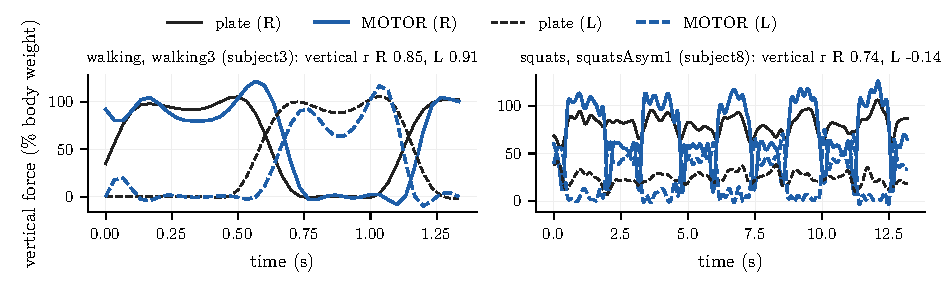
\includegraphics[width=\linewidth]{figures/grf.pdf}
\caption{Vertical force per foot against the plates, the 45\dg{} camera's median walking and squat trial, low-passed
as OpenCap scores them.}
\label{fig:grf}
\end{figure}

\paragraph{Time.} From the SOMA body to muscle forces MOTOR takes a median 66\,s per trial on one NVIDIA L4 (35 to
789\,s), against 2635 to 4196\,s for OpenCap's recorded solves on the CPU (Table~\ref{tab:timing}; models and
hardware differ). The run took at most 24 cards at once and EUR 29.5.
% labval-final-2026-11-07.txt ("sim body wall seconds per step", "run").

% #98 comment "Timing comparison" (OpenCap Setup.yaml/Stats.npy; Moco; CMC). MOTOR on SCORE clips:
% speed-2026-11-06.txt.


\section{Limitations}
% Elbow: paper/evidence/sim-body/elbow-2026-11-07.txt. Pelvis tilt, residuals, EMG channels:
% paper/evidence/sim-body/labval-final-2026-11-07.txt ("signed offsets", "residuals", "EMG per channel").

Four limits are measured and open. The elbows come out 21 to 24\dg{} straighter than the lab's in every envelope
trial (centred error 3 to 6\dg). The offset is GEM-X's arm estimate, not the sim body's: on 540 walking arm-trials
GEM-X's own elbow is a median 18.5\dg{} straighter than the lab's markers, and the sim body follows it within 2.5\dg. The pelvis tilt is biased
by about 5\dg{} (one direction in 82 of 89 envelope trials). The pelvis residual stays above OpenSim's limits (2\% body weight, 1\% weight times
centre-of-mass height; medians 7.0\% and 8.9\%), so the forces are not yet dynamically consistent with the movement. The activation pattern is
still partly off: rectus femoris does not follow its EMG ($r=-0.08$) and gluteus medius agrees on or off on only half
the frames. LabValidation is one small healthy cohort.

\section{Conclusion}

MOTOR gives foot forces, moments and 416 muscle forces from one video in a minute per trial on one GPU.

% Every float of the main body is placed before this point, so the page count below is honest.
\FloatBarrier
\label{endofmain}

\bibliographystyle{unsrtnat}
\bibliography{references}

\clearpage
\appendix
\section{Full technical validation}

Laid out as Appendix B of \cite{kardolus2026direct}. All 720 single-camera inputs (every activity including drop jumps,
each camera its own input) were prepared and sent to the cluster; 715 ran and were scored, and
Appendix~\ref{app:failures} gives the rest by cause. ``Before'' is the previous full run of the same 720 inputs (700
scored) with the chain as it was before the contact, ground and ligament changes, scored again with this run's code.
Every number is from paper/evidence/sim-body/labval-final-2026-11-07.txt.
% That file's "run" and header.

\subsection{Every joint angle}
\begin{center}\small
\captionof{table}{MAE and centred MAE (degrees) per coordinate, previous full run $\rightarrow$ this run, and this run's
mean $r$ ($^\dagger$: the reference moves less than 15\dg). Envelope: 45\dg{} camera, no drop jumps (72 $\rightarrow$
89 trials). All: every scored input (700 $\rightarrow$ 715). The matched 15 first; pro\_sup has no shared zero, so only
its cMAE.}
\begin{tabular}{@{}lcccccc@{}}
\toprule
 & \multicolumn{3}{c}{Envelope} & \multicolumn{3}{c}{All} \\
Coordinate & MAE & cMAE & $r$ & MAE & cMAE & $r$ \\
\midrule
ankle angle r & 6.41 $\rightarrow$ 6.39 & 3.18 $\rightarrow$ 3.19 & 0.89 & 5.97 $\rightarrow$ 5.96 & 3.94 $\rightarrow$ 3.92 & 0.92 \\
ankle angle l & 4.45 $\rightarrow$ 4.61 & 3.22 $\rightarrow$ 3.32 & 0.89 & 5.52 $\rightarrow$ 5.51 & 3.75 $\rightarrow$ 3.75 & 0.92 \\
knee angle r & 6.30 $\rightarrow$ 6.06 & 3.16 $\rightarrow$ 3.04 & 0.99 & 6.02 $\rightarrow$ 5.99 & 3.18 $\rightarrow$ 3.17 & 0.99 \\
knee angle l & 6.10 $\rightarrow$ 5.94 & 3.33 $\rightarrow$ 3.24 & 0.98 & 6.11 $\rightarrow$ 6.09 & 3.51 $\rightarrow$ 3.50 & 0.98 \\
hip flexion r & 8.17 $\rightarrow$ 8.03 & 3.90 $\rightarrow$ 3.82 & 0.98 & 8.91 $\rightarrow$ 8.89 & 4.16 $\rightarrow$ 4.11 & 0.98 \\
hip flexion l & 7.46 $\rightarrow$ 7.37 & 3.56 $\rightarrow$ 3.53 & 0.98 & 8.96 $\rightarrow$ 8.93 & 4.22 $\rightarrow$ 4.17 & 0.98 \\
hip adduction r & 4.20 $\rightarrow$ 4.20 & 2.81 $\rightarrow$ 2.73 & 0.52$^\dagger$ & 3.69 $\rightarrow$ 3.72 & 2.58 $\rightarrow$ 2.59 & 0.52$^\dagger$ \\
hip adduction l & 4.78 $\rightarrow$ 4.72 & 2.83 $\rightarrow$ 2.76 & 0.60$^\dagger$ & 3.48 $\rightarrow$ 3.52 & 2.50 $\rightarrow$ 2.52 & 0.57$^\dagger$ \\
hip rotation r & 4.10 $\rightarrow$ 4.07 & 2.62 $\rightarrow$ 2.62 & 0.43$^\dagger$ & 4.38 $\rightarrow$ 4.36 & 2.77 $\rightarrow$ 2.77 & 0.51 \\
hip rotation l & 4.53 $\rightarrow$ 4.41 & 3.19 $\rightarrow$ 3.06 & 0.43$^\dagger$ & 4.22 $\rightarrow$ 4.20 & 3.03 $\rightarrow$ 3.00 & 0.54 \\
pelvis tilt & 5.93 $\rightarrow$ 6.06 & 3.60 $\rightarrow$ 3.64 & 0.51 & 7.05 $\rightarrow$ 7.02 & 4.43 $\rightarrow$ 4.39 & 0.40 \\
pelvis list & 3.26 $\rightarrow$ 3.15 & 2.48 $\rightarrow$ 2.46 & 0.17$^\dagger$ & 3.10 $\rightarrow$ 3.11 & 2.22 $\rightarrow$ 2.24 & 0.16$^\dagger$ \\
lumbar extension & 4.66 $\rightarrow$ 4.56 & 3.15 $\rightarrow$ 3.11 & 0.64 & 5.36 $\rightarrow$ 5.32 & 3.37 $\rightarrow$ 3.35 & 0.75 \\
lumbar bending & 4.37 $\rightarrow$ 4.19 & 3.31 $\rightarrow$ 3.21 & 0.44 & 3.68 $\rightarrow$ 3.69 & 2.51 $\rightarrow$ 2.54 & 0.45$^\dagger$ \\
lumbar rotation & 3.67 $\rightarrow$ 3.67 & 2.14 $\rightarrow$ 2.12 & 0.58$^\dagger$ & 4.01 $\rightarrow$ 3.97 & 2.74 $\rightarrow$ 2.71 & 0.44 \\
\midrule
arm add l & 3.79 $\rightarrow$ 3.98 & 2.33 $\rightarrow$ 2.34 & 0.70 & 6.62 $\rightarrow$ 6.58 & 5.18 $\rightarrow$ 5.12 & 0.70 \\
arm add r & 4.30 $\rightarrow$ 4.23 & 2.25 $\rightarrow$ 2.23 & 0.51$^\dagger$ & 6.22 $\rightarrow$ 6.16 & 4.45 $\rightarrow$ 4.40 & 0.64 \\
arm flex l & 7.92 $\rightarrow$ 8.03 & 3.11 $\rightarrow$ 3.19 & 0.93 & 12.59 $\rightarrow$ 12.46 & 8.72 $\rightarrow$ 8.59 & 0.90 \\
arm flex r & 6.77 $\rightarrow$ 7.00 & 3.09 $\rightarrow$ 3.19 & 0.93 & 11.32 $\rightarrow$ 11.20 & 8.65 $\rightarrow$ 8.52 & 0.90 \\
arm rot l & 8.19 $\rightarrow$ 8.01 & 4.41 $\rightarrow$ 4.50 & 0.64 & 12.48 $\rightarrow$ 12.35 & 9.91 $\rightarrow$ 9.78 & 0.67 \\
arm rot r & 7.25 $\rightarrow$ 7.03 & 4.27 $\rightarrow$ 4.09 & 0.67 & 11.31 $\rightarrow$ 11.18 & 8.74 $\rightarrow$ 8.61 & 0.68 \\
elbow flex l & 23.80 $\rightarrow$ 23.68 & 4.74 $\rightarrow$ 4.61 & 0.74 & 24.77 $\rightarrow$ 24.70 & 5.73 $\rightarrow$ 5.67 & 0.79 \\
elbow flex r & 20.96 $\rightarrow$ 21.12 & 3.07 $\rightarrow$ 3.00 & 0.80 & 22.79 $\rightarrow$ 22.74 & 5.84 $\rightarrow$ 5.76 & 0.76 \\
mtp angle l & 15.23 $\rightarrow$ 15.35 & 2.49 $\rightarrow$ 2.47 & 0.15$^\dagger$ & 15.73 $\rightarrow$ 15.74 & 2.19 $\rightarrow$ 2.19 & 0.10$^\dagger$ \\
mtp angle r & 15.17 $\rightarrow$ 15.22 & 2.58 $\rightarrow$ 2.55 & -0.02$^\dagger$ & 14.99 $\rightarrow$ 14.99 & 2.05 $\rightarrow$ 2.06 & 0.00$^\dagger$ \\
pelvis rotation & 2.76 $\rightarrow$ 2.70 & 2.63 $\rightarrow$ 2.57 & 0.50$^\dagger$ & 2.66 $\rightarrow$ 2.63 & 2.45 $\rightarrow$ 2.42 & 0.48$^\dagger$ \\
pro sup l & - & 2.82 $\rightarrow$ 2.82 & 0.16$^\dagger$ & - & 3.63 $\rightarrow$ 3.61 & 0.25 \\
pro sup r & - & 2.44 $\rightarrow$ 2.55 & 0.18$^\dagger$ & - & 3.48 $\rightarrow$ 3.46 & 0.26$^\dagger$ \\
subtalar angle l & 9.18 $\rightarrow$ 9.24 & 7.02 $\rightarrow$ 6.88 & -0.21 & 9.74 $\rightarrow$ 9.73 & 6.25 $\rightarrow$ 6.25 & -0.07 \\
subtalar angle r & 9.02 $\rightarrow$ 9.16 & 6.26 $\rightarrow$ 6.26 & 0.04 & 11.44 $\rightarrow$ 11.39 & 6.21 $\rightarrow$ 6.21 & 0.04 \\
\midrule
matched 15, pooled & 5.23 $\rightarrow$ 5.16 & 3.10 $\rightarrow$ 3.06 & & 5.36 $\rightarrow$ 5.35 & 3.26 $\rightarrow$ 3.25 & \\
\bottomrule
\end{tabular}
\end{center}
The angles are the same chain's in both runs (GEM-X and the fit are unchanged); the small differences come from the
inputs each run has. The elbows are about 21 to 25\dg{} off with a centred error of 3 to 6\dg{} (straighter than the
lab's in each of the 89 envelope trials; GEM-X's arm estimate, which the sim body follows), and the toes (mtp)
15\dg{} off with a centred 2 to 3\dg: constant offsets, not tracking errors.

\subsection{Per subject group, activity and camera}
\begin{center}\small
\captionof{table}{This run per group (the previous full run's value in brackets): inputs, matched MAE and cMAE
(degrees), vertical GRF MAE (\% body weight, both feet), median vertical $r$ per foot, joint moment MAE over OpenCap's
15 (\% weight $\times$ height), mean EMG $r$ over the channels. Cameras: LabValidation's numbering; Cam1 is the envelope's 45\dg{} camera.}
\begin{tabular}{@{}lccccccc@{}}
\toprule
Group & $n$ & MAE & cMAE & GRF vert. & $r$ R / L & Moments & EMG $r$ \\
\midrule
held out 7--11 & 396 & 5.13 (5.14) & 3.02 (3.02) & 16.28 (54.33) & 0.77 / 0.79 & 2.41 (2.43) & 0.24 \\
training 2--5 & 319 & 5.62 (5.65) & 3.54 (3.56) & 16.15 (53.07) & 0.78 / 0.77 & 2.42 (2.48) & 0.22 \\
walking & 135 & 4.38 (4.40) & 2.92 (2.93) & 19.55 (76.11) & 0.82 / 0.80 & 1.88 (1.79) & 0.27 \\
walking (trunk sway) & 135 & 4.67 (4.67) & 3.05 (3.05) & 16.31 (84.14) & 0.82 / 0.84 & 1.72 (1.53) & 0.27 \\
squats & 87 & 5.79 (5.79) & 3.26 (3.28) & 6.32 (47.18) & 0.53 / 0.47 & 1.58 (1.54) & 0.17 \\
sit-to-stand & 90 & 5.39 (5.34) & 2.92 (2.91) & 11.58 (47.71) & 0.68 / 0.80 & 1.55 (1.74) & 0.20 \\
drop jump & 268 & 6.03 (6.03) & 3.63 (3.63) & 19.27 (32.21) & 0.78 / 0.78 & 3.59 (3.73) & 0.22 \\
Cam0 & 144 & 5.21 (5.20) & 3.14 (3.14) & 14.95 (54.10) & 0.75 / 0.83 & 2.44 (2.44) & 0.23 \\
Cam1 (45\dg) & 141 & 5.62 (5.72) & 3.33 (3.40) & 15.50 (53.27) & 0.73 / 0.81 & 2.54 (2.65) & 0.22 \\
Cam2 & 144 & 5.36 (5.36) & 3.53 (3.53) & 15.54 (52.72) & 0.81 / 0.82 & 2.21 (2.31) & 0.25 \\
Cam3 & 143 & 5.35 (5.35) & 3.20 (3.21) & 15.96 (53.03) & 0.81 / 0.70 & 2.44 (2.44) & 0.23 \\
Cam4 & 143 & 5.23 (5.23) & 3.05 (3.05) & 19.16 (55.68) & 0.78 / 0.75 & 2.43 (2.45) & 0.23 \\
\bottomrule
\end{tabular}
\end{center}

\subsection{Ground reaction force}
\begin{center}\small
\captionof{table}{Ground reaction force per activity, this run (previous run in brackets): MAE in \% body weight on
three axes with both feet summed, as OpenCap scored it; the share of the plate's stance frames the run's foot carries.}
\begin{tabular}{@{}lccccc@{}}
\toprule
Activity & vertical & anterior & medio-lateral & 3-axis mean & stance carried R / L \\
\midrule
all & 16.22 (53.77) & 7.41 (6.45) & 2.99 (3.19) & 8.9 (21.1) & 0.82 / 0.79 \\
walking & 19.55 (76.11) & 12.03 (9.65) & 3.02 (3.35) & 11.5 (29.7) & 0.82 / 0.75 \\
walking (trunk sway) & 16.31 (84.14) & 10.86 (9.11) & 3.49 (4.21) & 10.2 (32.5) & 0.83 / 0.85 \\
squats & 6.32 (47.18) & 3.53 (2.56) & 3.30 (4.17) & 4.4 (18.0) & 0.99 / 0.95 \\
sit-to-stand & 11.58 (47.71) & 4.42 (4.74) & 3.25 (3.51) & 6.4 (18.7) & 0.82 / 0.82 \\
drop jump & 19.27 (32.21) & 5.61 (5.37) & 2.54 (2.20) & 9.1 (13.3) & 0.76 / 0.71 \\
\midrule
OpenCap, 2 cameras & 11.4 & 3.5 & 3.8 & 6.2 & -- \\
\bottomrule
\end{tabular}
\end{center}

\subsection{Residuals}
\begin{center}\small
\captionof{table}{The pelvis residual this run leaves, per group: the median over trials of each trial's median force
(\% body weight) and moment (\% weight $\times$ centre-of-mass height), the median of each trial's 95th-percentile force,
and the mean share of frames within both of OpenSim's limits (2\% and 1\%). No trial is within them on every frame.}
\begin{tabular}{@{}lccccc@{}}
\toprule
Group & trials & force & moment & force, 95th pct. & frames within \\
\midrule
all & 715 & 7.0 & 8.90 & 24.4 & 21\% \\
held out 7--11 & 396 & 7.1 & 9.31 & 23.9 & 21\% \\
walking & 135 & 7.8 & 10.99 & 23.0 & 6\% \\
walking (trunk sway) & 135 & 7.0 & 9.59 & 20.3 & 7\% \\
squats & 87 & 0.7 & 1.06 & 8.4 & 49\% \\
sit-to-stand & 90 & 0.2 & 2.82 & 8.8 & 46\% \\
drop jump & 268 & 10.9 & 9.32 & 85.5 & 17\% \\
\bottomrule
\end{tabular}
\end{center}

\subsection{Muscle activations against EMG}
\begin{center}\small
\captionof{table}{Each EMG channel against MOTOR's activation of that muscle, all 715 inputs: the share of frames on
which both are on or both off, Pearson's $r$, and the lag (s) at the cross-correlation peak.}
\begin{tabular}{@{}lccc@{\hspace{2em}}lccc@{}}
\toprule
Muscle & on/off & $r$ & lag & Muscle & on/off & $r$ & lag \\
\midrule
bflh l & 0.65 & 0.13 & -0.130 & semiten r & 0.70 & 0.23 & -0.034 \\
bflh r & 0.65 & 0.13 & -0.144 & soleus l & 0.70 & 0.26 & -0.030 \\
gasmed l & 0.70 & 0.23 & -0.009 & soleus r & 0.69 & 0.28 & -0.041 \\
gasmed r & 0.69 & 0.26 & -0.022 & tibant l & 0.59 & 0.22 & +0.031 \\
glmed1 l & 0.51 & 0.13 & +0.051 & vaslat l & 0.72 & 0.40 & -0.003 \\
glmed1 r & 0.52 & 0.15 & +0.040 & vaslat r & 0.72 & 0.42 & -0.018 \\
recfem l & 0.56 & -0.08 & -0.002 & vasmed l & 0.72 & 0.36 & -0.024 \\
semiten l & 0.66 & 0.18 & -0.053 & vasmed r & 0.76 & 0.41 & -0.033 \\
\bottomrule
\end{tabular}
\end{center}

\begin{center}\small
\captionof{table}{OpenCap's vasti symmetry index in squats: the AUC of MOTOR's index against the asymmetry the
instructions asked for and against the EMG's own label (index over 1.15), previous run $\rightarrow$ this run.
OpenCap: 0.83 against the EMG label.}
\begin{tabular}{@{}lcc@{}}
\toprule
Camera & AUC, instructed & AUC, EMG label \\
\midrule
Cam0 & 0.47 $\rightarrow$ 0.84 & 0.64 $\rightarrow$ 0.75 \\
Cam1 & 0.52 $\rightarrow$ 0.72 & 0.08 $\rightarrow$ 0.62 \\
Cam2 & 0.60 $\rightarrow$ 0.95 & 0.52 $\rightarrow$ 0.84 \\
Cam3 & 0.75 $\rightarrow$ 0.90 & 0.65 $\rightarrow$ 0.83 \\
Cam4 & 0.53 $\rightarrow$ 0.81 & 0.25 $\rightarrow$ 0.48 \\
all & 0.56 $\rightarrow$ 0.73 & 0.45 $\rightarrow$ 0.66 \\
\bottomrule
\end{tabular}
\end{center}

\subsection{Time per step}
\begin{center}\small
\captionof{table}{MOTOR's sim body wall seconds per step on one NVIDIA L4, over the 715 runs: median, range, and the
median per frame (clips of 30\,Hz).}
\begin{tabular}{@{}lcccc@{}}
\toprule
Step & median s & min s & max s & s per frame \\
\midrule
fit & 21.825 & 14.483 & 623.317 & 0.303 \\
set up: Newton's model, its card, the filtered path & 4.697 & 3.878 & 32.851 & 0.061 \\
footing & 4.669 & 1.758 & 35.312 & 0.062 \\
RRA, rounds & 19.862 & 5.910 & 392.306 & 0.246 \\
RRA, follows and frame caps & 4.603 & 1.714 & 45.888 & 0.061 \\
checks: RRA's record, feet held, following on MuJoCo's compile & 2.120 & 1.111 & 17.879 & 0.028 \\
static optimisation 1, ground reaction & 3.003 & 0.114 & 28.318 & 0.034 \\
static optimisation 2, stops and muscles & 2.296 & 1.169 & 22.356 & 0.032 \\
inverse dynamics, contacts and muscle paths & 1.120 & 0.356 & 12.459 & 0.013 \\
records and push measures & 0.264 & 0.042 & 2.639 & 0.003 \\
arrays & 0.005 & 0.003 & 0.012 & 0.000 \\
total & 66.214 & 34.843 & 788.668 & 0.871 \\
\bottomrule
\end{tabular}
\end{center}


\begin{table}[h]
\centering\small
\caption{Wall time per trial. OpenCap's solves are from its LabValidation release (80 muscles, windows of 0.99 to
1.68\,s, solve only, hardware not recorded). Figure~\ref{fig:timing} draws them on one scale.}
\label{tab:timing}
\begin{tabular}{@{}lll@{}}
\toprule
Chain & Clip & Wall time \\
\midrule
OpenCap solve \cite{uhlrich2023opencap} & walk, drop jump, squat & 4196, 4096, 2635\,s \\
Moco, MocoTrack \cite{dembia2020moco} & gait & about 130\,min \\
OpenSim CMC \cite{rajagopal2016fullbody} & gait & about 10\,min \\
MOTOR sim body, one L4 & LabValidation, 715 trials & 66\,s median (35--789\,s) \\
\bottomrule
\end{tabular}
\end{table}

\begin{figure}[h]
\centering
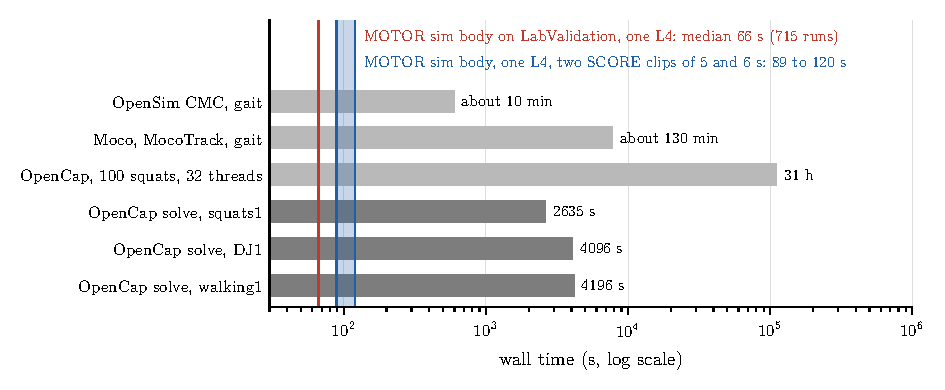
\includegraphics[width=\linewidth]{figures/timing.pdf}
\caption{Wall time per trial, log scale: OpenCap's recorded solves and published OpenSim times (grey), MOTOR's sim
body on two SCORE clips (blue band) and its median on LabValidation (red).}
\label{fig:timing}
\end{figure}

\begin{figure}[h]
\centering
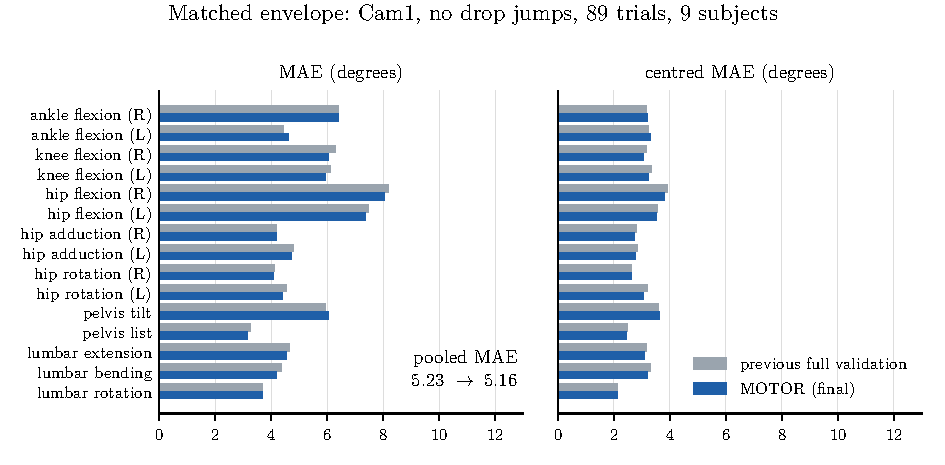
\includegraphics[width=\linewidth]{figures/angles-bars.pdf}
\caption{Per-coordinate MAE and centred MAE on the matched envelope, previous full run and this run.}
\label{fig:angles}
\end{figure}

\begin{figure}[h]
\centering
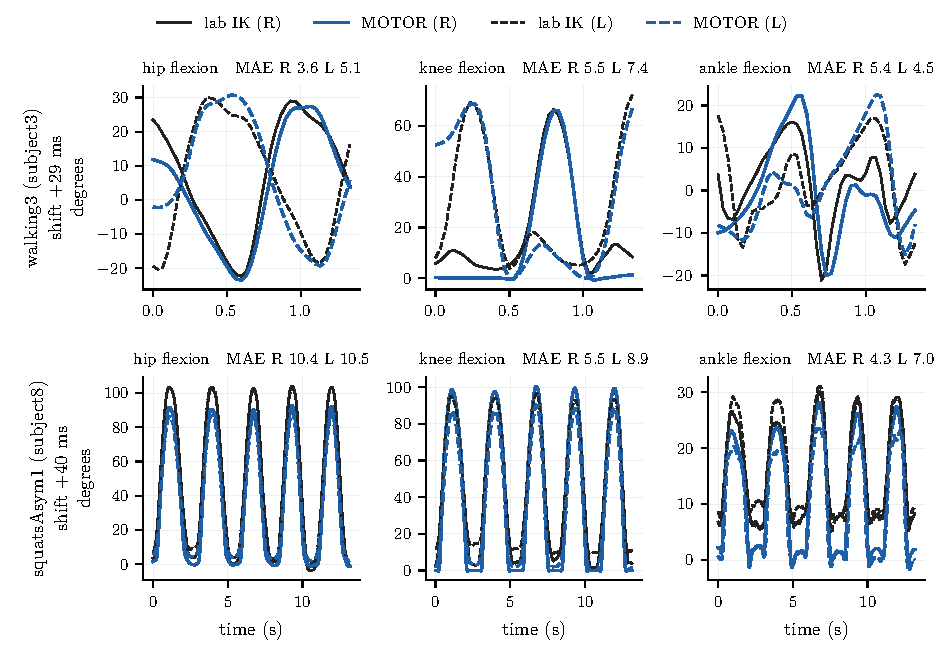
\includegraphics[width=\linewidth]{figures/waveforms.pdf}
\caption{Hip, knee and ankle flexion of the 45\dg{} camera's median walking and squat trial (by angle error), MOTOR
against the lab's inverse kinematics moved by the scored time shift.}
\label{fig:waveforms}
\end{figure}
\FloatBarrier

\section{Failures}
\label{app:failures}

\begin{center}\small
\captionof{table}{The 5 of 720 inputs without a score in this run, by cause.}
\begin{tabular}{@{}lr@{}}
\toprule
Cause & Inputs \\
\midrule
The card's fit solve did not stop in 3000 steps (subject 10, squats1, two cameras) & 2 \\
A frame's fit did not converge in 300 steps (two drop jumps) & 2 \\
Passed its job's time limit (subject 10, squats1, a third camera) & 1 \\
\midrule
Total & 5 \\
\bottomrule
\end{tabular}
\end{center}
The run first stopped at its EUR 25 spend limit with 3 of its 48 jobs unfinished; their 45 inputs ran after with the
same code.

Two faults found in the first scoring of an earlier run are fixed and reported because they moved the headline
number then. First, 148 of the 720 GEM-X results came from another video: a resumed cloud run named its jobs by
position in a shortened list, so a job picked up an earlier job's finished output; jobs are now named by a hash of
their own description. Second, the time shift could not reach a walking trial's true lag: requiring the shifted
reference to cover 80\% of a clip about one gait cycle long capped the shift near $\pm0.27$\,s, against the protocol's
$\pm1.0$\,s; at 50\% the feet are in phase at the found lag in every walking trial. The pooled matched MAE went from
8.59\dg{} (78 trials) to 6.02\dg{} (62 trials) then.
% labval-final-2026-11-07.txt ("run"); earlier faults: labval-diagnosis (#98), Causes 1 and 2 and the first table.

\section{Disclosure}

The code of MOTOR and of its validation was written by a coding agent (Claude Code) under the author's direction and
review; this draft was written the same way. No result was hand-picked. Three contact settings and the box
clearance were chosen on LabValidation's subjects 2 to 5 against their force plates, never against joint angles;
subjects 7 to 11 were held out and are reported apart. The figures' trials were picked by rule (the median trial by
angle error), not by eye.

\end{document}
